\subsection{Спектральный анализ}
Спектральный анализ - это один из методов обработки сигналов, который позволяет охарактеризовать частотный состав измеряемого сигнала.
Методы статистики играют важную роль в спектральном анализе, поскольку сигналы, как правило, имеют шумовой или случайный характер. Если бы
основные статистические характеристики сигнала были известны точно или же их можно было бы без ошибок определить на конечном интервале этого
сигнала, то спектральный анализ представлял бы собой отрасль точной науки. В действительности по одному-единственному отрезку сигнала можно
получить только некоторую оценку его спектра. Практика спектрального анализа после 1880-х гг. постепенно стала превращаться в некое ремесло
достаточно субъективного характера, которое на ряду с использованием научного подхода требовало также определенного уровня эмпирического
искусства \cite{marpl_book}.

\subsubsection{Применение нормального уравнения Юла-Уолкера}
В 1927 г. Дж. Юл предложил существенно новый метод спектрального анализа. Для отыскаяния одной-двух переодичностей в исследуемых данных Юл
прибег к моделированию временного ряда, основанному на линейном регрессионном анализе. Юла интересовала главным образом более высокая точность
определения основной периодичности в ряде чисел солнечных пятен и отыскания в нем дополнительных периодичностей \cite{marpl_book}.
Используя простое тригонометрическое тождество:
\begin{center}
\begin{equation}
	\label{eq:yule_trigonometric}
	\sin(kx)=2\cos(x)\sin([k-1]x)-sin([k-2]x)
\end{equation}
\end{center}
Используя подстановки и обобщая формулу (весь ход обобщения описан в \cite{marpl_book}) можно получить:
\begin{center}
\begin{equation}
	\label{eq:yule_raznost}
	u(k) = b(1)u(k-1) + b(2)u(k-2) + \epsilon (k)
\end{equation}
\end{center}
Здесь ${u(k) = \sin (2\pi fkT)}$ - гармоническая составляющая, ${T}$ - интервал отсчетов, ${f}$ - частота гармоник, а
${b(1)}$ и ${b(2)}$ принимают произвольные значения. Как легко увидеть, уравнение \ref{eq:yule_raznost} представляет собой АР уравнение, и это был
первый случай когда АР по методу наименьших квадратор применялась для целей спектроанализа. Решением уравнения \ref{eq:yule_raznost}
является затухающая синусойда.

АР модель предсказания отсчета может быть описана как взвешенная сумма ${P}$ предыдущих отсчетов сигнала:
\begin{center}
\begin{equation}
	\label{eq:lpc_forecast}
	\hat{x(m)} = \sum \limits_{i=1}^P a_k x(m-k),
\end{equation}
\end{center}
Где ${\hat{x(m)}}$ - оценка ${x(m)}$ в момент времени ${m}$, а ${a_k}$ - коэффициенты АР модели.

Оценка ошибки ${e(m)}$ может быть представлена как:
\begin{center}
\begin{equation}
	\label{eq:lpc_error}
	e(m) = x(m) - \hat{x(m)} = x(m) - \sum \limits_{i=1}^P a_k x(m-k),
\end{equation}
\end{center}

Из уравнения \ref{eq:lpc_error} смоделированный сигнал может быть представлен следующим рекурсивным соотношением:
\begin{center}
\begin{equation}
	\label{eq:lpc_signal}
	x(m) = \sum \limits_{i=1}^P a_k x(m-k) + e(m)
\end{equation}
\end{center}

Уравнения \ref{eq:lpc_error} представляет собой цифровой фильтр.
После ${z}$ - преобразования уравнение \ref{eq:lpc_signal} может быть записана как \cite{saeed_book}:
\begin{center}
\begin{eqnarray}
	\label{eq:lpc_z}
		H(z)	& = & \frac{X(z)}{U(z)} = \frac{G}{1 - \sum \limits_{k=1}^P a_kz^{-k}} =  \nonumber \\
			& = & G\frac{1}{\prod \limits_{k=1}^N (1-r_kz^{-1})} \frac{1}{\prod \limits_{k=1}^M (1-2r_k \cos \phi_k z^{-1} + r_k^2z^{-2})}
\end{eqnarray}
\end{center}

В уравнении \ref{eq:lpc_z} ${M}$ - пары комплексных полюсов, ${N}$ - действиьедбные полюсы с ${P=N+2M}$,
${r_k}$ и ${\phi_k}$ - радиус и угол ${k}$ - го полюса соответственно. Частотный ответ такой системы 
может быть представлен \cite{saeed_book}:
\begin{center}
\begin{eqnarray}
	\label{eq:lpc_freq_resp}
		H(f)	& = & = \frac{G}{1 - \sum \limits_{k=1}^P a_k e^{-j2 \pi kf}} =  \nonumber \\
			& = & G\frac{1}{\prod \limits_{k=1}^N (1-r_k e^{-j2 \pi f)}} \frac{1}{\prod \limits_{k=1}^M (1-2r_k \cos \phi_k e^{-j2 \pi f} + r_k^2 e^{-j4 \pi f})}
\end{eqnarray}
\end{center}

Уравнения, соответствующие линейному предсказанию, по своей структуре идентичны уравнениям Юла-Уолкера для АР-процесса.
В виду этого существует тесная связь между фильтром линейного предсказания и АР-процессом \cite{marpl_book}.

На рисунке \ref{pic:lpc_poles} изображено отношение между полюсами и АЧХ рекурсивного фильтра. На частотах, соответствующих полюсам,
на графике АЧХ присутствуют частотные пики. Пары комплексных корней могут быть представлены через радиус ${r_k}$ и угол ${\phi_k}$
полюса:

\begin{center}
\begin{equation}
	\label{eq:lpc_poles}
	z_k = r_k e^{\pm j \phi_k}
\end{equation}
\end{center}

Резонансные частоты выражаются через комплексные полюса как:
\begin{center}
\begin{equation}
	\label{eq:lpc_poles_freq}
	F(\phi_k)=\frac{F_s}{2 \pi} \phi_k
\end{equation}
\end{center}
где ${F_s}$ - частота оцифровки.

\begin{figure}[H]
	\center\scalebox{1}{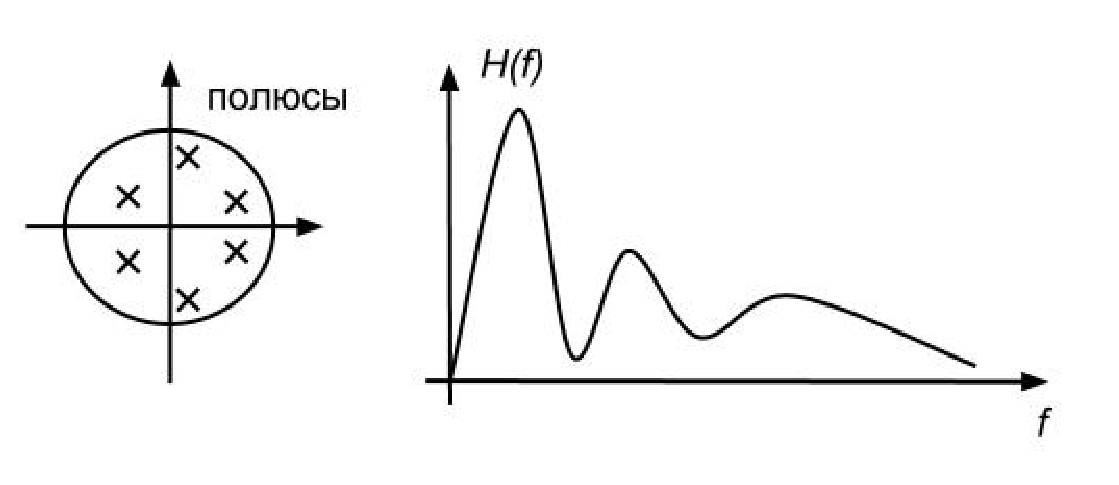
\includegraphics[width=1\linewidth]{lpc_poles.eps}}
	\caption{Полюса и АЧХ линейного предсказателя}
	\label{pic:lpc_poles}
\end{figure}

\paragraph{Вычисление коэффициентов АР модели}
Наилучшие оценки коэффициентов ${a_k}$ могут быть получены минимизацией среднеквадратичной ошибки уравнения\cite{saeed_book}
\ref{eq:lpc_error}:
\begin{center}
\begin{eqnarray}
	\label{eq:lpc_rms}
		E[e^2(m)]	& = & E[(x(m) - \sum \limits_{i=1}^P a_k x(m-k))^2] =\nonumber \\
				& = & E[x^2(m)] - \nonumber \\
				& &  - 2\sum \limits_{i=1}^P a_k E[x(m-k)x(m)] + \nonumber \\
				& &  + \sum \limits_{i=1}^P a_k \sum \limits_{j=1}^P a_j E[x(m-k)x(m-j)] = \nonumber \\
				& = & r_{xx}(0) - 2{\bf r}^T_{xx}{bf a} + {\bf a}^T {\bf R_{xx}a}
\end{eqnarray}
\end{center}
Где ${{\bf R_{xx}} = E[{\bf xx}^T]}$ - это автокорреляционная матрица входного вектора ${{\bf x}^T=[x(m-1),x(m-2),...,x(m-P)]}$,
${{\bf r}_{xx}=E[x(m){\bf x}]}$ - автокорреляционный вектор, а ${a^T=[a_1,a_2,...,a_P]}$ -  вектор коэффициентов предсказателя.
Минимизация среднеквадратичной ошибки из уравнения \ref{eq:lpc_rms} может быть записано как:
\begin{center}
\begin{equation}
	\label{eq:lpc_rms2}
	{\bf a=R^{-1}_{xx}r_{xx}}
\end{equation}
\end{center}

Можно использовать альтернативную запись.
Для сигнала длинной в ${N}$ семплов можно записать ${N}$ - уравнений:
\begin{center}
\begin{equation}
	\label{eq:lpc_rms3}
	{\bf e=x-Xa}
\end{equation}
\end{center}
Уравнение \ref{eq:lpc_rms3} можно переписать в виде:
\begin{center}
\begin{equation}
	\label{eq:lpc_rms4}
	{\bf eу^T = xx^T - 2x^T Xa + a^T X^T Xa}
\end{equation}
\end{center}

Взяв производную по вектору ${{\bf a}}$, можно получить параметры предсказателя:
\begin{center}
\begin{equation}
	\label{eq:lpc_rms5}
	\frac{\partial {\bf e^T e}}{\partial {\bf a}} = {\bf - 2x^T X + a^T X^T X} = 0
\end{equation}
\end{center}
Из \ref{eq:lpc_rms6}, коэффициенты для минимальной среднеквадратичной ошибки равны:
\begin{center}
\begin{equation}
	\label{eq:lpc_rms6}
	{\bf a= (X^T X)^{-1} (X^T x)}
\end{equation}
\end{center}

Из сравнения уравнений \ref{eq:lpc_rms2} и \ref{eq:lpc_rms6} видно, что в \ref{eq:lpc_rms2}
автокорреляционная матрица и вектор заменены оценками:
\begin{center}
\begin{equation}
	\label{eq:lpc_rms7}
	\hat{r_{xx}}(m) = \frac{1}{N} \sum \limits_{k=0}^{N-1} x(k)x(k-m)
\end{equation}
\end{center}

Уравнения \ref{eq:lpc_rms2} и \ref{eq:lpc_rms7} могут быть эффиктивно решены с помощью регулярных
Тёплицевых структур корреляционной матрицы ${{\bf R_{xx}}}$. Эффективным алгоритмам над Тёплицевыми
матрицами посвещена книга \cite{bleyhut_book} (а это нужно????) Эффективным методом решения
данных соотношений является алгоритм Левинсона-Дарби.

АР метод оценивания СПМ часто используется для того, чтобы выявить в данных наличие синусоидальных
компонент. Мощность, соответствующую  таким компонентам в АР оценке СПМ, можно вычислить, интегрируя
площадь под кривой этой оценки. Однако это связано с большими вычислительными затратами, поэтому
гораздо более эффективным является использования в качестве показателя мощности синусоидальных
компонент высоты соответствующих им спектральных пиков \cite{marpl_book}.  

\newpage
